\begin{frame}[fragile]{Visualização da soma das submatrizes a partir dos valores de $p$}

    \begin{figure}[!h]
        \centering
        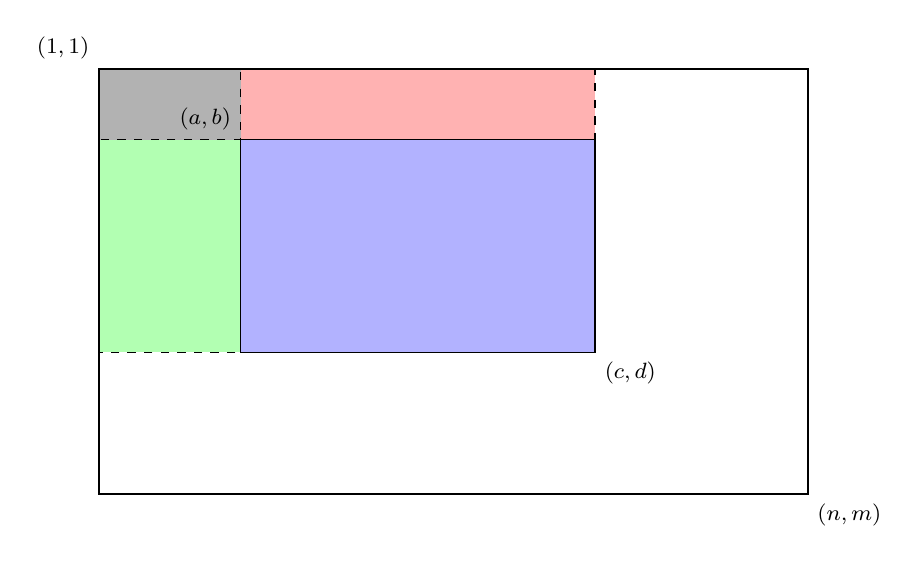
\begin{tikzpicture}[scale=0.9]
            \draw[dashed,fill=red!30] (0, 5) rectangle (7, 6);
            \draw[dashed,fill=green!30] (0, 2) rectangle (2, 6);
            \draw[dashed,fill=black!30] (0, 5) rectangle (2, 6);
            \draw[fill=blue!30] (2, 2) rectangle (7, 5);
            \draw[thick] (0, 0) rectangle (10, 6);

            \node[anchor=north west] at (7, 2) { \footnotesize $(c, d)$ };
            \node[anchor=south east] at (2, 5) { \footnotesize $(a, b)$ };
            \node[anchor=south east] at (0, 6) { \footnotesize $(1, 1)$ };
            \node[anchor=north west] at (10, 0) { \footnotesize $(n, m)$ };
        \end{tikzpicture}
    \end{figure}

\end{frame}
